% Options for packages loaded elsewhere
\PassOptionsToPackage{unicode}{hyperref}
\PassOptionsToPackage{hyphens}{url}
%
\documentclass[
]{article}
\usepackage{amsmath,amssymb}
\usepackage{lmodern}
\usepackage{iftex}
\ifPDFTeX
  \usepackage[T1]{fontenc}
  \usepackage[utf8]{inputenc}
  \usepackage{textcomp} % provide euro and other symbols
\else % if luatex or xetex
  \usepackage{unicode-math}
  \defaultfontfeatures{Scale=MatchLowercase}
  \defaultfontfeatures[\rmfamily]{Ligatures=TeX,Scale=1}
\fi
% Use upquote if available, for straight quotes in verbatim environments
\IfFileExists{upquote.sty}{\usepackage{upquote}}{}
\IfFileExists{microtype.sty}{% use microtype if available
  \usepackage[]{microtype}
  \UseMicrotypeSet[protrusion]{basicmath} % disable protrusion for tt fonts
}{}
\makeatletter
\@ifundefined{KOMAClassName}{% if non-KOMA class
  \IfFileExists{parskip.sty}{%
    \usepackage{parskip}
  }{% else
    \setlength{\parindent}{0pt}
    \setlength{\parskip}{6pt plus 2pt minus 1pt}}
}{% if KOMA class
  \KOMAoptions{parskip=half}}
\makeatother
\usepackage{xcolor}
\IfFileExists{xurl.sty}{\usepackage{xurl}}{} % add URL line breaks if available
\IfFileExists{bookmark.sty}{\usepackage{bookmark}}{\usepackage{hyperref}}
\hypersetup{
  pdftitle={Variational Monte Carlo studies of bosonic systems},
  pdfauthor={Anna Stray Rongve; Knut Magnus Aasrud; Amund Midtgard Raniseth},
  hidelinks,
  pdfcreator={LaTeX via pandoc}}
\urlstyle{same} % disable monospaced font for URLs
\usepackage{longtable,booktabs,array}
\usepackage{calc} % for calculating minipage widths
% Correct order of tables after \paragraph or \subparagraph
\usepackage{etoolbox}
\makeatletter
\patchcmd\longtable{\par}{\if@noskipsec\mbox{}\fi\par}{}{}
\makeatother
% Allow footnotes in longtable head/foot
\IfFileExists{footnotehyper.sty}{\usepackage{footnotehyper}}{\usepackage{footnote}}
\makesavenoteenv{longtable}
\setlength{\emergencystretch}{3em} % prevent overfull lines
\providecommand{\tightlist}{%
  \setlength{\itemsep}{0pt}\setlength{\parskip}{0pt}}
\setcounter{secnumdepth}{5}
\usepackage{graphicx}
\usepackage{subfig}
\usepackage{placeins}
\makeatletter
\newcommand*{\centerfloat}{%
  \parindent \z@
  \leftskip \z@ \@plus 1fil \@minus \textwidth
  \rightskip\leftskip
  \parfillskip \z@skip}
\makeatother
\ifLuaTeX
  \usepackage{selnolig}  % disable illegal ligatures
\fi
\newlength{\cslhangindent}
\setlength{\cslhangindent}{1.5em}
\newlength{\csllabelwidth}
\setlength{\csllabelwidth}{3em}
\newenvironment{CSLReferences}[2] % #1 hanging-ident, #2 entry spacing
 {% don't indent paragraphs
  \setlength{\parindent}{0pt}
  % turn on hanging indent if param 1 is 1
  \ifodd #1 \everypar{\setlength{\hangindent}{\cslhangindent}}\ignorespaces\fi
  % set entry spacing
  \ifnum #2 > 0
  \setlength{\parskip}{#2\baselineskip}
  \fi
 }%
 {}
\usepackage{calc}
\newcommand{\CSLBlock}[1]{#1\hfill\break}
\newcommand{\CSLLeftMargin}[1]{\parbox[t]{\csllabelwidth}{#1}}
\newcommand{\CSLRightInline}[1]{\parbox[t]{\linewidth - \csllabelwidth}{#1}\break}
\newcommand{\CSLIndent}[1]{\hspace{\cslhangindent}#1}

\title{Variational Monte Carlo studies of bosonic systems}
\author{Anna Stray Rongve \and Knut Magnus Aasrud \and Amund Midtgard
Raniseth}
\date{\today}

\begin{document}
\maketitle

\begin{abstract}
We use Rust to develop a ground state solver for bosonic systems in an elliptical harmonic trap, utilizing the variational principle, Monte Carlo integration and two different implementations of the Metropolis-Hastings algorithm. The results are compared against each other and analytical solutions for the corresponding systems. The solver gives the desired results, but shows instability for the importance sampling Metropolis algorithm.
\end{abstract}

\hypertarget{introduction}{%
\section{Introduction}\label{introduction}}

Finding the ground state properties of a trapped hard sphere Bose-gas
can be a difficult task to do analytically, but has great relevancy in
investigating gases of alkali atoms, as stated by DuBois and Glyde
{[}1{]}. As such, we shall implement a variational Monte Carlo solver
specialized for the problem at hand, and solve it numerically. This is
done in Rust, a fast, safe and modern compiled language.

We will investigate a simple boson gas situated in an elliptical
harmonic potential well. This is done by employing the variational
principle (as explained by Griffiths {[}2{]}) to find the optimal wave
function and corresponding energy. We consider both the case of
non-interacting particles, described by their single particle Gaussian
wave function, and also expand this model to interacting systems by
introducing the Jastrow function for pairwise interaction. Using the
Metropolis-Hastings algorithm paired with Monte Carlo integration, we
calculate the expected local energy of the system and use steepest
gradient descent to find the minimum of this energy with regards to the
variational parameter \(\alpha\).

In this report, we will first introduce the theory behind our approach
and find an analytical solution for a simplified system. This is done to
have a benchmark to which we can compare the performance of our
numerical solver. Thereafter we present the methodology behind our
solver and how its implemented. The results it produces and comparisons
are shown in section \ref{results} and further discussed in section
\ref{discussion}.

\hypertarget{theory}{%
\section{Theory}\label{theory}}

The system in question is a hard sphere Bose gas located in a potential
well. The potential is an \emph{elliptical harmonic trap}, described for
each particle by

\begin{equation}V_\text{ext}(\mathbf r) = \frac{1}{2}m\left(\omega_\text{ho}^2(r_x^2 + r_y^2) + \omega_z^2 r_z^2\right).\label{eq:external-potential}\end{equation}

Here, \(\mathbf r\) is the position of the particle and
\(\omega_\text{ho}\) is the frequency of the trap. Note that setting
\(\omega_\text{ho} = \omega_z\) results in eq.
\eqref{eq:external-potential} evaluating to
\(V_\text{ext}(\mathbf r) = \frac{1}{2}m\omega_\text{ho}^2r^2\), which
represents the \emph{spherical} case of the elliptical harmonic trap. As
a simplification, we hereby denote the spherical case as (S) and the
general elliptical case as (E).

In addition to this external potential, we represent the inter-boson
interactions with the following pairwise, repulsive potential{[}3{]}:

\begin{equation}V_\text{int}(|\mathbf r_i - \mathbf r_j|) = \begin{cases}\infty & |\mathbf r_i - \mathbf r_j| \le a \\ 0 & |\mathbf r_i - \mathbf r_j| > a\end{cases},\label{eq:internal-potential}\end{equation}

where \(a\) is the hard-core diameter of the bosons. Eq.
\eqref{eq:external-potential} and eq. \eqref{eq:internal-potential}
evaluate to the following two-body Hamiltonian:

\begin{equation}H = \sum_i^N\left(-\frac{\hbar^2}{2m}\nabla_i^2 + V_\text{ext}(\mathbf r_i)\right) + \sum_{i < j}^N V_\text{int} (|\mathbf r_i - \mathbf r_j|).\label{eq:hamiltonian}\end{equation}

The term \(-\frac{\hbar^2}{2m}\nabla_i^2\) stems from the kinetic energy
of the system and the index notation used is described in
\ref{index-notation-for-sums-and-products}. By scaling into length units
of \(a_\text{ho}\) and energy units of \(\hbar\omega_\text{ho}\), this
equation is further simplified into:

\begin{equation} H = \frac{1}{2}\sum_i^N \left(-\nabla_i^2 + r_{x, i}^2 + r_{y, i}^2 + \gamma^2 r_{z, i}^2\right) + \sum_{i<j}^N V_\text{int}(|\mathbf r_i - \mathbf r_j|) ,\label{eq:scaled_ham}\end{equation}

where \(\gamma = \frac{\omega_z}{\omega_\text{ho}}\). The derivation of
\eqref{eq:scaled_ham} is explained in \ref{sec:scaled_ham}. Lastly we
also define the so-called local energy, which is the quantity we want to
integrate over to find the total energy of the system:

\begin{equation} E_L(\mathbf r) = \frac{1}{\Psi_T(\mathbf r)}H\Psi_T(\mathbf r) \label{eq:local-energy}\end{equation}

\hypertarget{the-variational-principle}{%
\subsection{The variational principle}\label{the-variational-principle}}

Given the above Hamiltonian, we can introduce the concept of a
\emph{trial wave function} \(\Psi_T(\alpha)\). This is a normalized
ansatz to the ground state wave function, parametrized by the
parameter(s) \(\alpha\). This gives us a way of deploying the
\emph{variational principle} by varying said parameter \(\alpha\) to our
needs:

We know that for any normalized function \(\Psi_T\), the expected energy
is higher than the ground state energy (as proved by Griffiths {[}2{]}
on p.~293-294), viz.

\begin{equation} \langle E(\alpha) \rangle = \langle \Psi_T(\alpha) | H | \Psi_T(\alpha)\rangle \ge E_0 = \langle \Psi_0 | H | \Psi_0\rangle. \label{eq:variational-principle}\end{equation}

Thus, minimizing over \(\alpha\) will give an approximation of the true
ground state (perhaps even an accurate answer).

Evaluating this integral is computationally demanding. Hence, we utilize
Monte Carlo integration to allow scalability. This is done by changing
the particles positions where the shifting follows some rules. For each
change, the local energy is sampled resulting in an expectation value of
the energy \(\langle E\rangle\) for the Hamiltonian.

To find the lowest value with regards to \(\alpha\), we could either
test over many different values, or use gradient descent methods. The
latter requires an expression for
\(\frac{\partial E}{\partial \alpha}\), which we choose to define
thusly:

\[ \dot E_\alpha = \frac{\partial \langle E_L(\alpha)\rangle}{\partial \alpha} .\]

Using the additional notation of
\(\dot \Psi_{T, \alpha} = \frac{\partial \langle \Psi_T(\alpha)\rangle}{\partial \alpha}\),
it can be shown that by using the chain rule and the hermiticity of the
Hamiltonian {[}4{]}, we get the expression

\begin{equation} \dot E_\alpha = 2\left(\left\langle\frac{\dot \Psi_{T, \alpha}}{\Psi(\alpha)} E_L(\alpha)\right\rangle - \left\langle\frac{\dot \Psi_{T, \alpha}}{\Psi(\alpha)}\right\rangle \langle E_L(\alpha)\rangle\right) \label{eq:energy-deriv}\end{equation}

Further explanation on how this is used in our gradient descent method
is explained in the section
\protect\hyperlink{steepest-gradient-descent}{Steepest gradient
descent}.

\hypertarget{wave-function}{%
\subsection{Wave function}\label{wave-function}}

For \(N\) particles, we use the following trial wave function:

\begin{equation}\Psi_T(\mathbf r_1, ..., \mathbf r_N, \alpha, \beta) = \prod_i g(\alpha, \beta, \mathbf r_i) \prod_{j < k}f(a, |\mathbf r_j - \mathbf r_k|)\label{eq:trial-wavefunction}\end{equation}

Once again, the index notation is described in
\ref{index-notation-for-sums-and-products}. Here we've used that

\begin{align*}
g(\alpha,\beta,\mathbf{r}_i) &= e^{-\alpha(x_i^2+y_i^2+\beta z_i^2)}, \\
\text{and }f(a,|\mathbf r_i-\mathbf r_j|) &= \begin{cases} 0 & |\mathbf r_i-\mathbf r_j| \le a \\ 1-\frac{a}{|\mathbf r_i-\mathbf r_j|} & {|\mathbf r_i-\mathbf r_j|} > a \end{cases},
\end{align*}

as shown in {[}3{]}. Simplifying the trial wave function can prove
useful, in order to reduce the number of floating point operations. An
analytical expression is also convenient for comparison with the
numerical calculations.

\hypertarget{importance-sampling}{%
\subsection{Importance sampling}\label{importance-sampling}}

Importance sampling, compared to the brute force Metropolis sampling,
sets a bias on the sampling, leading it on a better path. This means
that the desired standard deviation is acquired after fewer Monte Carlo
cycles.

For our quantum mechanical scenario with boson particles in a magnetic
trap, the bias has its root in the so-called quantum force. This quantum
force pushes the walker (the boson particle) to the regions where the
trial wave function is large. It is clear that this yields a faster
convergence compared to the Metropolis algorithm, where the walker has
the same probability of moving in all directions.

The quantum force \(\mathbf{F}\) is given by the formula

\[ \mathbf{F}=2 \frac{1}{\Psi_{T}} \nabla \Psi_{T}, \]

which is derived from the Fokker-Planck equation, using the Langevin
equation to generate the next step with Euler's method, and by making
the probability density converge to a stationary state.

\hypertarget{fokker-planck}{%
\subsubsection{Fokker-Planck}\label{fokker-planck}}

For one particle (or walker), the one-dimensional Fokker-Planck equation
for a diffusion process is:

\[ \frac{\partial P}{\partial t}=D \frac{\partial}{\partial x}\left(\frac{\partial}{\partial x}-F\right) P(x, t) \]

Where \(P(x,t)\) is a time-dependent probability density, \(D\) is the
diffusion coefficient and \(F\) is a drift term which in our case is
driven by the quantum force.

\hypertarget{langevin-equation}{%
\subsubsection{Langevin equation}\label{langevin-equation}}

The Langevin equation solution gives the position of the walker in the
next timestep. The Langevin equation is:

\[ \frac{\partial x(t)}{\partial t}=D F(x(t))+\eta \]

Converting this to a function yielding the new position \(y\) in a
computational manner, we use Euler's method.

\begin{equation} y=x+D F(x) \Delta t+\xi \sqrt{\Delta t} .\label{eq:euler_method}\end{equation}

Here \(x\) is the old position, \(y\) is the new position and \(\xi\) is
a randomly sampled value from the normal distribution. In scaled units,
the diffusion coefficient evaluates to \(\frac{1}{2}\). The timestep
\(\Delta t\) has stable values within the range
\(\Delta t \in [0.001, 0.01]\) , so we'll simply choose the value
\(\Delta t = 0.005\) here.

\hypertarget{fokker-planck-and-langevin-equation-in-importance-sampling}{%
\subsubsection{Fokker-Planck and Langevin equation in importance
sampling}\label{fokker-planck-and-langevin-equation-in-importance-sampling}}

In order to use these equations for our importance sampling, we start
with the original Fokker-Planck equation.

After inserting \(D\) as the diffusion coefficient and
\(\mathbf{F}_{\mathbf{i}}\) as component \(i\) of the drift velocity, we
can make the probability density converge to a stationary state by
setting its partial derivative over time to zero.

\[ \frac{\partial P}{\partial t}=\sum_{i} D \frac{\partial}{\partial \mathbf{x}_{\mathbf{i}}}\left(\frac{\partial}{\partial \mathbf{x}_{\mathbf{i}}}-\mathbf{F}_{\mathbf{i}}\right) P(\mathbf{x}, t) \]

Where then \(\frac{\partial P}{\partial t}= 0\), and by expanding the
parenthesis and moving the double partial derivative over to the other
side, we obtain:

\[ \frac{\partial^{2} P}{\partial \mathbf{x}_{\mathbf{i}}^{2}}=P \frac{\partial}{\partial \mathbf{x}_{\mathbf{i}}} \mathbf{F}_{\mathbf{i}}+\mathbf{F}_{\mathbf{i}} \frac{\partial}{\partial \mathbf{x}_{\mathbf{i}}} P \]

By inserting \(g(\mathbf{x}) \frac{\partial P}{\partial x}\) for the
drift term, \(\mathbf{F}\), we get

\[ \frac{\partial^{2} P}{\partial \mathbf{x} _{\mathbf{i}}{}^{2}}=P \frac{\partial g}{\partial P}\left(\frac{\partial P}{\partial \mathbf{x}_{i}}\right)^{2}+P g \frac{\partial^{2} P}{\partial \mathbf{x}_{i}^{2}}+g\left(\frac{\partial P}{\partial \mathbf{x}_{i}}\right)^{2} \]

Where again the left hand side can be set to zero to comply with the
fact that at a stationary state, the probability density is the same for
all walkers.

For this to be solvable, the remaining terms have to cancel each other.
This is only possible when \(g = P^{-1}\), which gives the aformentioned
quantum force, \(\mathbf{F},\)

\[ \mathbf{F}=2 \frac{1}{\Psi_{T}} \nabla \Psi_{T}. \]

From here, The Green's function is deployed as

\[ G(y, x, \Delta t)=\frac{1}{(4 \pi D \Delta t)^{3 N / 2}} \exp \left(\frac{-(y-x-D \Delta t F(x))^{2}}{ 4 D \Delta t}\right) \]

Which will be part of the proposal distribution, \(q(y,x)\) as

\begin{equation} q(y, x)=\frac{G(x, y, \Delta t)\left|\Psi_{T}(y)\right|^{2}}{G(y, x, \Delta t)\left|\Psi_{T}(x)\right|^{2}}\label{eq:proposal_distr}\end{equation}

\hypertarget{analytical-derivations}{%
\subsection{Analytical derivations}\label{analytical-derivations}}

\hypertarget{local-energy-simple-gaussian-wave-function}{%
\subsubsection{Local energy simple Gaussian wave
function}\label{local-energy-simple-gaussian-wave-function}}

As a test case to be compared against our numerical implementation, we
want to find an analytical expression for the energy of the trial wave
function. We simplify by studying only the non-interacting part, which
is done by setting the parameter \(a = 0\). We also set \(\beta = 1\),
giving us the following trial wave function:

\[\Psi_T(\mathbf{r_1, r_2,\ldots,r_N, \alpha, \beta}) = \prod_i \exp(-\alpha r_{i}^2).\]

Considering \eqref{eq:local-energy}:

\begin{align*}
E_L(\mathbf{r}) &=  \frac{1}{\Psi_T (\mathbf{r})} H \Psi_T (\mathbf{r})
= \frac{1}{\Psi_T (\mathbf{r})} \left[ \sum_i^N \left( \frac{-\hbar^2}{2m}
   \nabla_{i}^2 + V_{\text{ext}}({\mathbf{r}}_i)\right)  \right]\Psi_T(\mathbf{r}) \\
&= \frac{1}{\Psi_T(\mathbf{r})} \left[ \sum_i^N \left (\frac{-\hbar^2}{2m}
  \nabla_{i}^2 \Psi_T (\mathbf{r}) + V_\text{ext} ({\mathbf{r}}_i) \Psi_T(\mathbf{r}) \right) \right].
\end{align*}

We simplify \(\nabla_i^2\Psi_T\) as shown in
\ref{second-derivative-of-trial-wave-function}, yielding

\begin{equation}\nabla^2\Psi_t(\mathbf r) = -2\alpha\Psi_T\left(\dim - 2\alpha\mathbf r_i^2\right),\label{eq:second-derivative-of-trial-wave-function}\end{equation}

where \(\dim\) is the dimension of the system (1, 2 or 3). Given eq.
\eqref{eq:second-derivative-of-trial-wave-function}, we find that the
local energy for N particles in the case of the simple Gaussian
wavefunction is

\begin{equation} E_L(\mathbf{r}) = \frac{\hbar^2 }{m} \alpha N \dim +  \left( \frac{1}{2} m \omega^2_\text{ho} - 2 \alpha^2\right)  \sum_i^N \mathbf{r}^2_{i},\label{eq:local-energy-gauss}\end{equation}

as shown in \ref{local-energy-for-gaussian-wave-function}. We can
simplify this even further by scaling, namely setting \(\hbar = m = 1\),
which gives us the equation

\begin{equation}E_L(\mathbf{r}) = N\alpha  \dim  + \left(\frac{1}{2} \omega^2_\text{ho} - 2 \alpha^2\right) \sum_i^N \mathbf{r}^2_{i}\label{eq:local-energy-gauss-scaled}\end{equation}

An even simpler analytic expression is obtained by setting
\(\omega_{\text{ho}} = 1\) and taking the derivate of the local energy
with respect to \(r_i\), giving \(\alpha= 0.5\).

\begin{equation}E_L = \frac{N \dim}{2}\label{eq:local-energy-min}\end{equation}

\hypertarget{drift-force}{%
\subsubsection{Drift force}\label{drift-force}}

The following expression for the drift force will be used to
\textbf{explanation}

\[ F = \frac{2 \nabla_k \Psi_T(\mathbf{r})}{\Psi_T(\mathbf{r})} = -4 \alpha \mathbf{r}_{k} \]

applying the gradient operator to the trial wavefunction is already
shown (appendix: Second derivative of trial wave function).

\hypertarget{local-energy-for-full-wave-function}{%
\subsubsection{Local energy for full wave
function}\label{local-energy-for-full-wave-function}}

With \(\beta \ne 0\) and \(\text{a} > 0\) the wave function becomes a
bit more complicated as the potential/Gaussian can be can now be
elliptical and the wave function contains the Jastrow factor. The energy
is given as:

\[ E(\mathbf{r}) = \frac{1}{\Psi_T(\mathbf{r})}\sum_i^{N}\nabla_i^2\Psi_T(\mathbf{r}), \]

To simplify coming equations, we set
\(\phi(\mathbf r) = g(\alpha, \beta, \mathbf r)\),
\(u(r_{ij}) = \ln f(r_{ij})\) and \(r_{ij} = |r_i - r_j|\). With eq.
\eqref{eq:trial-wavefunction}, this results in

\[\Psi_T(\mathbf{r})=\prod_i^N \phi(\mathbf{r}_i) \exp{\left(\sum_{i<j}u(r_{ij})\right)}\]

Using this simplification, we show in \ref{sec:trial_wf_gradient} that
the gradient for the \(k\)-th particle is equal to:

\begin{align*} 
\nabla_k \Psi_T (\mathbf{r}) =\ &\nabla_k \phi (\mathbf{r}_ 4k)\left[\prod^N_{i \ne k}{\phi(\mathbf{r}_ k)} \right] \exp \left( \sum^N _{j<m} u(r _{jm})\right) \\ &+ \left[\prod^N _i\phi(\mathbf{r}_ i)\right] \exp \left( \sum^N _ {j<m} u(r _ {jm})\right) \sum^N _ {l\ne k } \nabla_ k (r_ {kl}).
\end{align*}

Furthermore, using the resulting Laplacian found in
\ref{sec:trial_wf_laplacian}, we can find

\begin{align*}
\frac{1}{\Psi_T(\mathbf{r})} \nabla_k^2 \Psi_T(\mathbf{r}) &= \frac{\nabla_k \phi(\mathbf{r}_k)}{\phi(\mathbf{r}_k)} + 2 \frac{\nabla_k \phi(\mathbf{r}_k)}{\phi(\mathbf{r}_k)}\sum _{j\ne k}
\frac{\mathbf{r}_j - \mathbf {r}_k}{\mathbf{r} _{jk}}u'(r _{lk})\\
&+ \sum _{j\ne k}\sum _{l\ne k}
\frac{\mathbf{r}_j - \mathbf {r}_k}{\mathbf{r} _{jk}} u'(r _{lk}) \\
&+ \sum _{j\ne k}\sum _{l\ne k}
\frac{\mathbf{r}_j - \mathbf {r}_k}{\mathbf{r} _{jk}} \frac{\mathbf{r}_l - \mathbf {r}_k}{\mathbf{r} _{lk}}  u'(r _{jk})  u'(r _{lk}) \\
&+ \sum _{l\ne k} \frac{2}{r _{lk}} u'(r _{lk}) +  u''(r _{lk})
\end{align*}

where these hold:

\begin{align*}
\frac{\nabla_k \phi(\mathbf{r}_k)}{\phi(\mathbf{r}_k)} &= -2\alpha \left[
\begin{matrix}
x_k^2 \\ y_k^2 \\ \beta z_k^2
\end{matrix}\right], \\ \\
\frac{\nabla_k^2 \phi(\mathbf{r}_k)}{\phi(\mathbf{r}_k)} &= 2\alpha (2\alpha)[x_k^2 + y_k^2 + \beta^2z_k^2] - 2 - \beta),\\ \\
u'(r_{ij}) &= \frac{r_{ij}}{r_{ij}-a}, \quad \text{for}  \quad r_{ij}  > a, \\ \\
u''(r_{ij}) &= \frac{a(a-2r_{ij})}{r_{ij}^2(a-r_{ij})^2}, \quad \text{for} \quad r_{ij}  > a.
\end{align*}

\hypertarget{one-body-density}{%
\subsubsection{One Body density}\label{one-body-density}}

The probability of finding a particle at a ceratin position is given by
the one body density. The probability is given by the following
integral.

\begin{align*}
  \rho(x_1) = \int{|\Psi(x_1, x_2,...|^2 dx_2 ...dx_N}
\end{align*}

Hence te probaility is given by the integral over all dimensions exept
the one in question.The integral gives a distrubution of all the
particles in question.

For a system with only a few particles, this would be hard to solve.
Approximating the integral using Monte Carlo integration, is however a
much simpler job.

\hypertarget{method}{%
\section{Method}\label{method}}

\hypertarget{variational-monte-carlo}{%
\subsection{Variational Monte Carlo}\label{variational-monte-carlo}}

\hypertarget{metropolis-sampling}{%
\subsubsection*{Metropolis sampling}\label{metropolis-sampling}}
\addcontentsline{toc}{subsubsection}{Metropolis sampling}

Since normalizing the wave function is computationally demanding, we
need another way of drawing samples from it. This is where the
Metropolis algorithm comes in.

For a given distribution \(p(\theta)\), we know that:

\[p(\theta) \propto g(\theta),\]

where our goal is to sample from \(p(\theta)\). The Metropolis algorithm
proceeds as follows:

\begin{enumerate}
\def\labelenumi{\arabic{enumi}.}
\tightlist
\item
  Select an initial value \(\theta_0\). This is often chosen randomly.
\item
  To produce a new sample:

  \begin{enumerate}
  \def\labelenumii{\arabic{enumii}.}
  \tightlist
  \item
    Draw a candidate \(\theta'\) from the proposal distribution
    \(q(\theta'|\theta_{i-1})\)
  \item
    Compute the ratio
    \(r = \frac{g(\theta')q(\theta_{i-1}|\theta')}{g(\theta_{i-1})q(\theta'|\theta_{i-1})}\)
  \item
    Decide:

    \begin{itemize}
    \tightlist
    \item
      If \(r \ge 1\) or \(r > u\) (where \(u\) is a random sample from
      the uniform distribution), set \(\theta_{i} = \theta'\).
    \item
      Else, set \(\theta_{i} = \theta_{i-1}\)
    \end{itemize}
  \end{enumerate}
\item
  Repeat as many times as needed.
\end{enumerate}

Our distribution \(p\) here is of course \(\Psi_T\). The proposal
distribution \(q(\theta'|\theta_{i-1})\) is the distribution that
suggests a new sample given the previous one. In the case which we'll
call the \emph{brute force Metropolis}, our choice here is the normal
distribution centered around the previous sample to favor samples close
to it. This makes the sequence into a random walk and our \(r\) becomes
a bit simpler, namely \(r = \frac{g(\theta')}{g(\theta_{i-1})}\). A flaw
with this is that the sampler might not converge around the important
parts\footnote{Namely the greater values of the distribution, which
  actually contribute.} and jump around a bit ``willy-nilly.'' To combat
this, we utilize the proposal distribution shown in eq.
\eqref{eq:proposal_distr} to get more relevant samples quicker. We will
use the term \emph{importance sampling Metropolis} to refer to this
method.

\hypertarget{monte-carlo-integration}{%
\subsubsection*{Monte Carlo integration}\label{monte-carlo-integration}}
\addcontentsline{toc}{subsubsection}{Monte Carlo integration}

To evaluate the required integrals and find the energy, we use Monte
Carlo integration (see section 2.3.1 of our previous work {[}5{]}).
Instead of sampling randomly, we use the Metropolis algorithm as
explained above to get our new samples.

\hypertarget{steepest-gradient-descent}{%
\subsubsection*{Steepest gradient
descent}\label{steepest-gradient-descent}}
\addcontentsline{toc}{subsubsection}{Steepest gradient descent}

Lastly, to reach the optimum value of \(\alpha\), we wish to find the
minimum of \(E(\alpha)\), in tune with the variational principle as
shown in \ref{the-variational-principle}. This is achieved using a
simple steepest gradient descent (or SDG) method. Briefly explained, it
works by following the negative value of the gradient, which always
points in the direction of greatest momentaneous descent. So it proceeds
as follows:

\begin{equation} \alpha_{i+1} = \alpha_i - \eta \dot E_\alpha,\label{eq:sgd}\end{equation}

where \(\dot E_\alpha\) is the gradient of the energy with regards to
\(\alpha\) as defined in \eqref{eq:energy-deriv} and \(\eta\) is the
so-called \emph{learning rate} - a value which decides how big of a leap
we want to do in the direction of the negative gradient.

\hypertarget{numerical-differentiation}{%
\subsubsection*{Numerical
differentiation}\label{numerical-differentiation}}
\addcontentsline{toc}{subsubsection}{Numerical differentiation}

To numerically calculate the Laplacian (for use in evaluating the
kinetic energy), we use the second order central difference
approximation, namely

\[\frac{d^2 f(x)}{dx^2} \approx \frac{f(x-h) -2f(x) + f(x+h)}{h^2},\]

for sufficiently small \(h\).

\hypertarget{statistical-analysis}{%
\subsection{Statistical analysis}\label{statistical-analysis}}

\hypertarget{blocking}{%
\subsubsection*{Blocking}\label{blocking}}
\addcontentsline{toc}{subsubsection}{Blocking}

All of these computer simulations can be considered ``computational
experiments,'' and can thus be statistically analyzed in the same way as
real-life experiments. There is one catch, however: All our samples are
correlated with the previous one, making a ``correlation chain'' of
sorts. Nilsen {[}6{]} presents that in the case of correlated samples,
the standard deviation of a sampled quantity (in our case \(E\)) is

\[ \sigma_E = \sqrt{\frac{1 + 2\tau /\Delta t}{n - 1}\left(\langle E^2\rangle - \langle E\rangle^2\right)}, \]

where \(\Delta t\) is the time between each sample and \(\tau\) is the
time between one sample and the next uncorrelated sample - called the
\emph{correlation time}. To combat this correlation effect, we need to
split our samples into blocks, each containing \(N_\text{blocking}\)
samples. Assuming the blocks are big enough that they are uncorrelated,
we can calculate the variance normally based on their mean.

A natural value for \(N_\text{blocking}\) would be \(\tau\), but we
don't know it's value. A computationally efficient way of finding it is
to plot the standard deviation against different values of
\(N_\text{blocking}\). The error will initially increase, but eventually
plateau, by which we've reached uncorrelated samples and subsequently
our desired value for \(N_\text{blocking}\) {[}6{]}. Using this, we can
confidently compute the variance of our Monte Carlo integration.

\hypertarget{natural-length-scale}{%
\subsection{Natural length scale}\label{natural-length-scale}}

As shown in \ref{sec:scaled_ham}, we use scaled length-units of
\(r \rightarrow r' = \frac{r}{a_0}\) and
\(E \rightarrow E' = \frac{E}{\hbar \omega_\text{ho}}\). This gives us
the constants of \(a_0 = \frac{a}{a_\text{ho}}\) and
\(\gamma = \frac{\omega_z}{\omega_\text{ho}}\). These scaled units are
used throughout the program and are later reversed to get real values.

\hypertarget{choice-of-programming-language}{%
\subsection{Choice of programming
language}\label{choice-of-programming-language}}

The Variational Monte Carlo solver is implemented in Rust. The reasons
for choosing this language are two-fold:

\begin{itemize}
\tightlist
\item
  Rust is known for being on par with C/C++ in regards to efficiency.
  This makes it a great fit for heavy numerical computation, which is
  needed in a task like this.
\item
  In contrast with C/C++, Rust has guaranteed memory safety. This does
  of course not solve any logical errors in our code, but it alleviates
  a lot of the memory struggles often met when dealing with such a
  low-level language - especially with regards to parallellization.
\end{itemize}

In addition to these, we were all very intrigued by this modern language
that is currently taking the computer science world by storm.

\hypertarget{auto-vectorization}{%
\subsubsection{Auto-vectorization}\label{auto-vectorization}}

Auto-vectorization in Rust is almost as easy as in C++, and can be
applied by setting
\texttt{RUSTFLAGS\ =\ "-C\ opt-level=3\ -C\ target-cpu=native"} in the
\texttt{Cargo.toml} file, which basically inputs the parameters to the
compiler at compiletime. The first flag tells the compiler to run all
possible optimizations. Setting \texttt{opt-level=2} is the same as
running the alias \texttt{-O} which only runs some optimizations
{[}7{]}. \texttt{target-cpu} tells the compiler which cpu to compile
specific code for. By inserting \texttt{native}, the compiler will
compile for the cpu the compiler is run at {[}7{]}.

However, simple loops like \texttt{for\ i\ in\ 0..n} will not be
properly vectorized due to the fact that the compiler cannot guarantee
that the length of the loop is within bounds of the slice iterated over.
The easiest way to ensure that this does not happen is to use an
iterator. If this cannot be done, hinting to LLVM the length of the
slice would also eliminate the bound checks. An example is to define the
slice as \texttt{let\ x\ =\ \&x{[}0..n{]};}.

\hypertarget{results}{%
\section{Results}\label{results}}

\hypertarget{analytic-vs.-numerical-calulcations}{%
\subsection{Analytic vs.~numerical
calulcations}\label{analytic-vs.-numerical-calulcations}}

In order to test our algorithm for both the brute force and the
importance sampling algorithm, the results are compared to the
analytically calculated energy for a range of \(\alpha\)-values. It is
expected that the local energy is at its minimum at \(\alpha = 0.5\), as
shown in \eqref{eq:local-energy-min}, so the analytical graph
representing this equation should intersect our numerically calculated
energies in their minimum point. Figure \ref{fig:BF_vs_IM_VS_analytical}
shows a collection of graphs, most of them showing just this.

\begin{figure}[ht]%
  \centerfloat
  \captionsetup[subfigure]{labelformat=empty}
   \subfloat[]{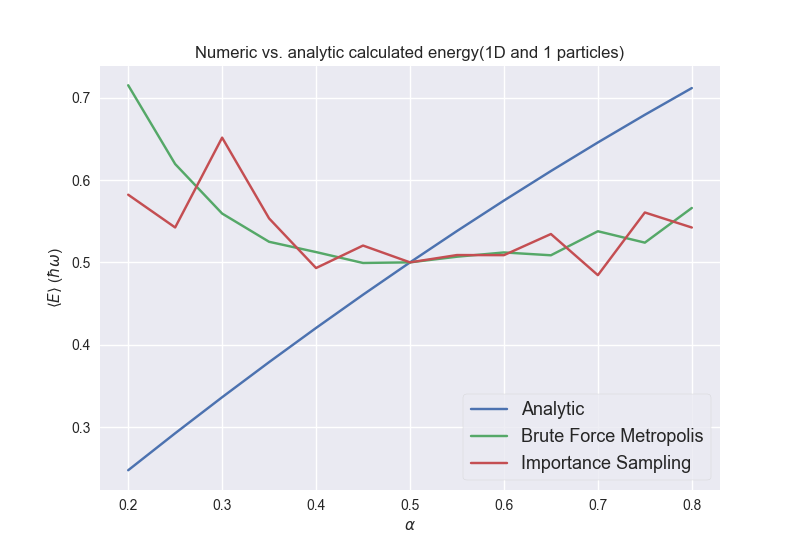
\includegraphics[scale=.5]{assets/plots/ana_vs_num/1D_1N/EnergyAlpha_BF_1D_1N.png}}
  \subfloat[]{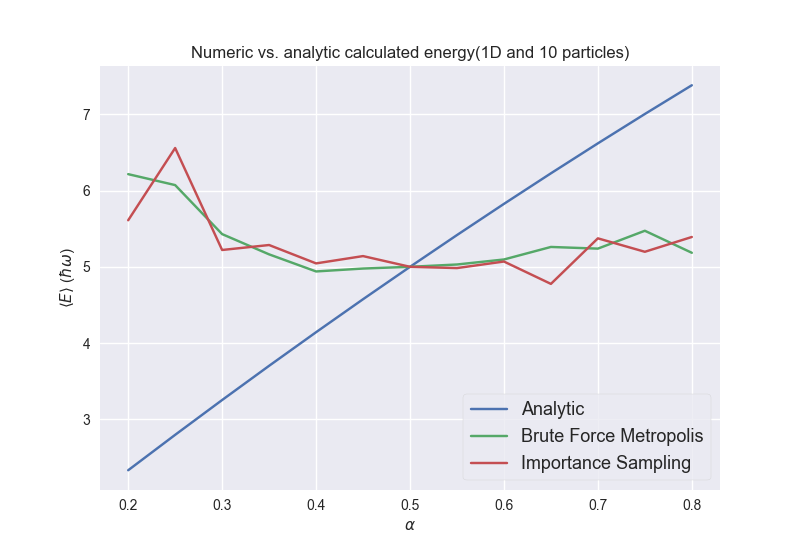
\includegraphics[scale=.5]{assets/plots/ana_vs_num/1D_10N/EnergyAlpha_BF_1D_10N.png}}\\
  \subfloat[]{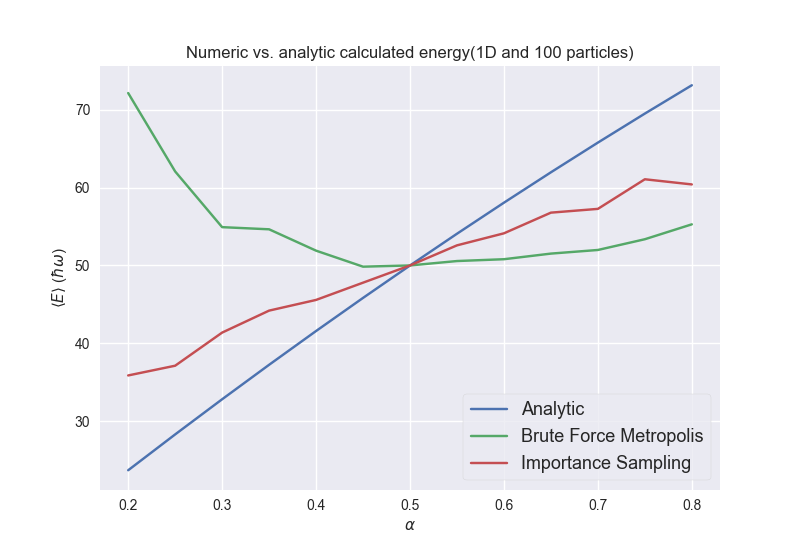
\includegraphics[scale=.5]{assets/plots/ana_vs_num/1D_100N/EnergyAlpha_BF_1D_100N.png}}
  \caption{Local energy (in units of $\hbar\omega_\text{ho}$), found at $N=1,10,100$  and for $\dim= 1$. The system is non-interacting and the values are calculated with both the brute force method, importance sampling and analytically.}
  \label{fig:BF_vs_IM_VS_analytical_1D}
\end{figure}

\begin{figure}[ht]%
  \centerfloat
  \captionsetup[subfigure]{labelformat=empty}
  \subfloat[]{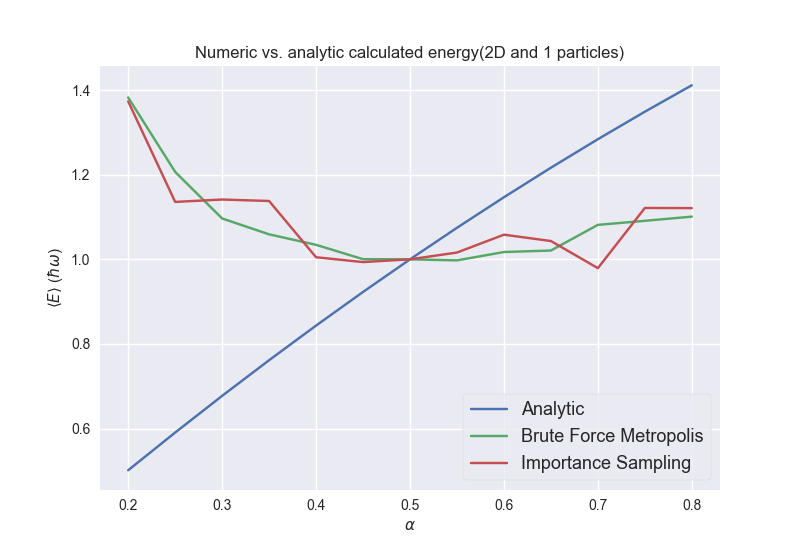
\includegraphics[scale=.5]{assets/plots/ana_vs_num/2D_1N/EnergyAlpha_BF_2D_1N.png}}
  \subfloat[]{
\includegraphics[scale=.5]{assets/plots/ana_vs_num/2D_10N/EnergyAlpha_BF_2D_10N.png}}\\
  \subfloat[]{
\includegraphics[scale=.5]{assets/plots/ana_vs_num/2D_100N/EnergyAlpha_BF_2D_100N.png}}
  \caption{Local energy (in units of $\hbar\omega_\text{ho}$), found at $N=1,10,100$  and for $\dim= 2$. The system is non-interacting and the values are calculated with both the brute force method, importance sampling and analytically.}
  \label{fig:BF_vs_IM_VS_analytical_2D}
\end{figure}

\begin{figure}[ht]%
  \centerfloat
  \captionsetup[subfigure]{labelformat=empty}
  \subfloat[]{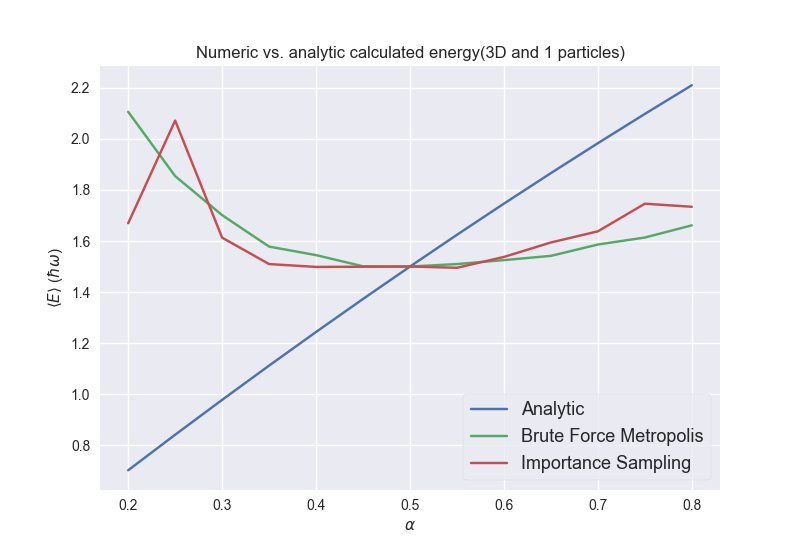
\includegraphics[scale=.5]{assets/plots/ana_vs_num/3D_1N/EnergyAlpha_BF_3D_1N.png}}
  \subfloat[]{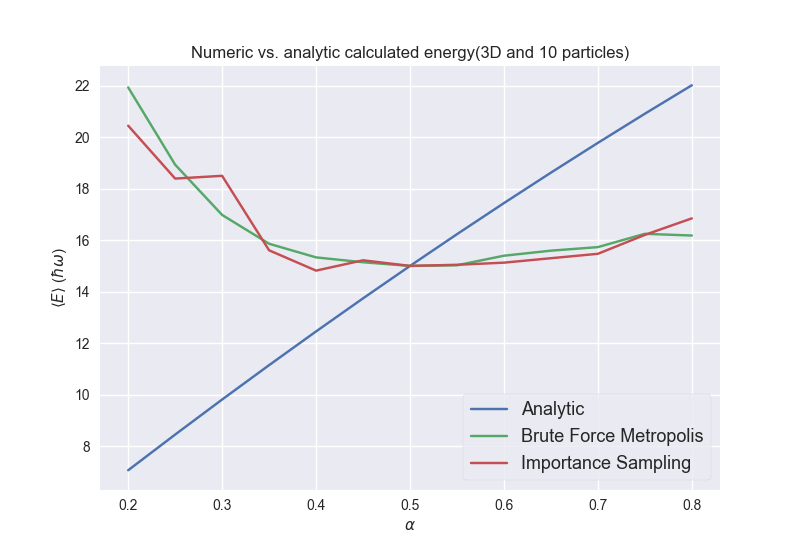
\includegraphics[scale=.5]{assets/plots/ana_vs_num/3D_10N/EnergyAlpha_BF_3D_10N.png}}\\
  \subfloat[]{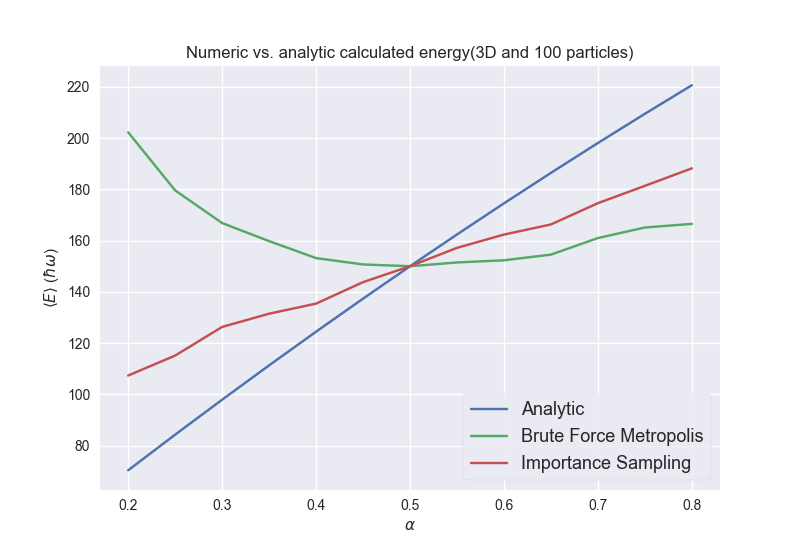
\includegraphics[scale=.5]{assets/plots/ana_vs_num/3D_100N/EnergyAlpha_BF_3D_100N.png}}
  \subfloat[]{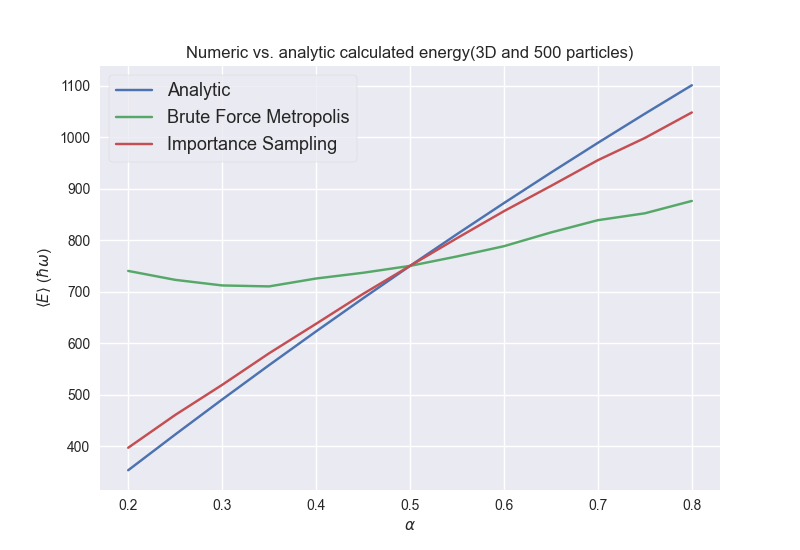
\includegraphics[scale=.5]{assets/plots/ana_vs_num/3D_500N/EnergyAlpha_BF_3D_500N.png}}
  \caption{Local energy (in units of $\hbar\omega_\text{ho}$), found at $N=1,10,100, 500$ (500 for 3D only - because of long computational time)  and for $\dim= 3$. The system is non-interacting and the values are calculated with both the brute force method, importance sampling and analytically.}
  \label{fig:BF_vs_IM_VS_analytical_3D}
\end{figure}

The total elapsed times of the three methods evaluating the simple
Gaussian wave function are listed in the table
\ref{tbl:BF_vs_IM_VS_analytical} below.

\begin{longtable}[]{@{}lccc@{}}
\caption{Total time (in seconds) to calculate the local energy for
\(\alpha = 0.5\) with the specified parameters: \(D\) dimensions and
\(N\) number of particles. Computation times are presented for the brute
force Metropolis algorithm, the importance sampling algorithm and the
analytical exact energy (the first two in Rust, the latter in Python).
\label{tbl:BF_vs_IM_VS_analytical}}\tabularnewline
\toprule
& \textbf{Brute force} & \textbf{Importance sampling} &
\textbf{Analytic} \\
\midrule
\endfirsthead
\toprule
& \textbf{Brute force} & \textbf{Importance sampling} &
\textbf{Analytic} \\
\midrule
\endhead
\(D=1, N=1\) & \(0.23\) & \(0.58\) & \(0.0\) \\
\(D=1, N=10\) & \(1.47\) & \(1.68\) & \(0.0\) \\
\(D=1, N=100\) & \(90.4\) & \(109\) & \(0.016\) \\
\(D=2, N=1\) & \(0.22\) & \(0.36\) & \(0.0\) \\
\(D=2, N=10\) & \(2.73\) & \(3.45\) & \(0.0041\) \\
\(D=2, N=100\) & \(186\) & \(233\) & \(0.009\) \\
\(D=3, N=1\) & \(0.33\) & \(0.40\) & \(0.0\) \\
\(D=3, N=10\) & \(2.95\) & \(3.71\) & \(0.001\) \\
\(D=3, N=100\) & \(161\) & \(214\) & \(0.004\) \\
\(D=3, N=500\) & \(3990\) & \(5280\) & \(0.02\) \\
\bottomrule
\end{longtable}

\hypertarget{finding-the-optimal-alpha}{%
\subsection{\texorpdfstring{Finding the optimal
\(\alpha\)}{Finding the optimal \textbackslash alpha}}\label{finding-the-optimal-alpha}}

Using the brute force Metropolis algorithm, we calculated the expected
value of the local energy at different values of \(\alpha\). This was
also done at different dimensions and number of particles. The
simulation over all these variables were done once for each core of the
processor running them. In our case, this resulted in 8 runs. The mean
over all runs are seen in figure \ref{fig:optimal_alpha}.

\begin{figure}[ht]%
  \centerfloat
  \captionsetup[subfigure]{labelformat=empty}
  \subfloat[]{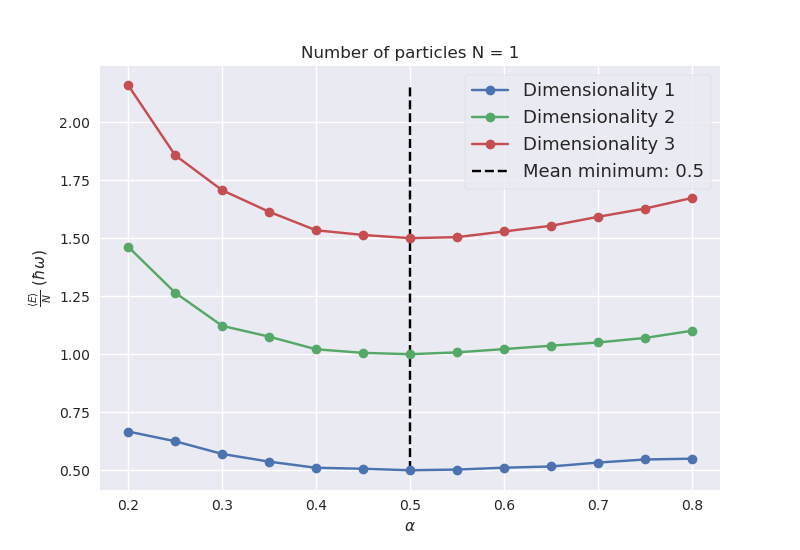
\includegraphics[scale=.5]{assets/plots/dim_and_n/EnergyAlpha_1.0N.png}}
  \subfloat[]{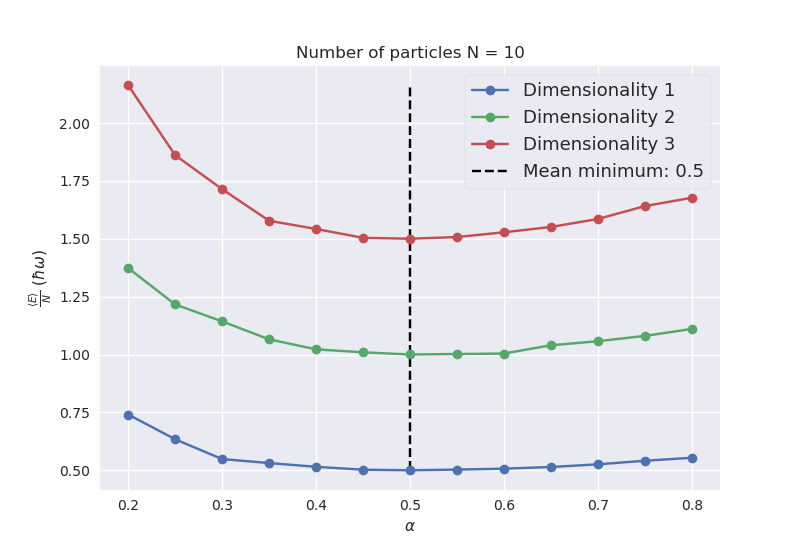
\includegraphics[scale=.5]{assets/plots/dim_and_n/EnergyAlpha_10.0N.png}}\\
  \subfloat[]{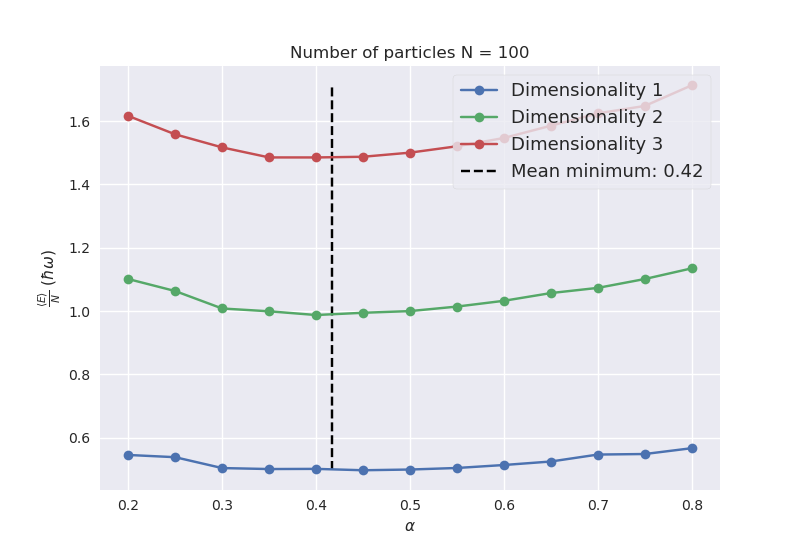
\includegraphics[scale=.5]{assets/plots/dim_and_n/EnergyAlpha_100.0N.png}}
  \caption{Expected local energy (in units of $\hbar\omega_\text{ho}$) per particle, found at $N=1,10,100$ and for $\dim= 1,2,3$. The results are the means over simulations run on 8 CPU cores simultaneously. The black dashed line shows the mean minimum over all three dimensions. The system is non-interacting and the values are calculated with the brute force method.}
  \label{fig:optimal_alpha}
\end{figure}

In figure \ref{fig:optimal_alpha}, we see that the optimal value of
\(\alpha\) seems to be consistently on the value \(0.5\), as expected.
However, for \(N = 100\) the mean deviates a bit from our expectation. A
more telling picture appears when we plot the standard deviation over
the CPU cores as a function of \(\alpha\) instead of the expected local
energy. This is shown in figure \ref{fig:optimal_alpha_std}. From this
its much more clear that we're reaching the actual desired\footnote{Desired
  because having a low standard deviation suggests that we've approached
  the true value.} value of \(\alpha\) at \(0.5\), regardless of how
many number of particles we're simulating for.

\begin{figure}[ht]%
  \centerfloat
  \captionsetup[subfigure]{labelformat=empty}
  \subfloat[]{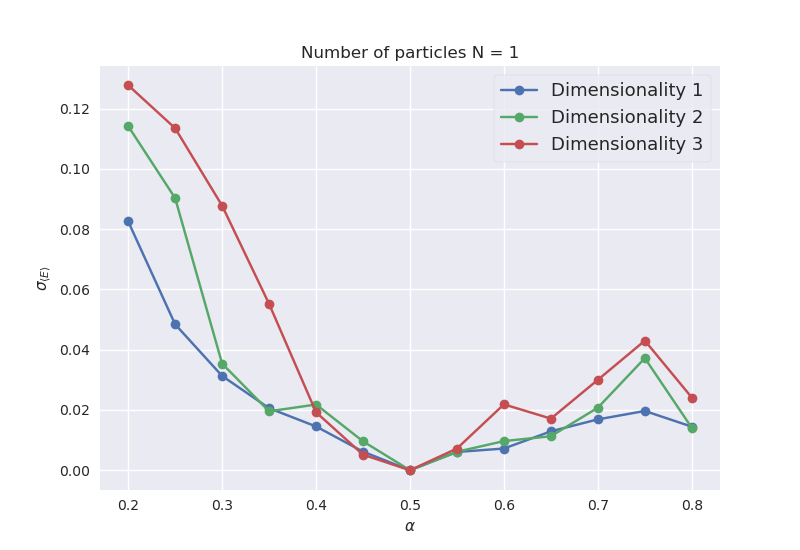
\includegraphics[scale=.5]{assets/plots/dim_and_n/std_1.0N.png}}
  \subfloat[]{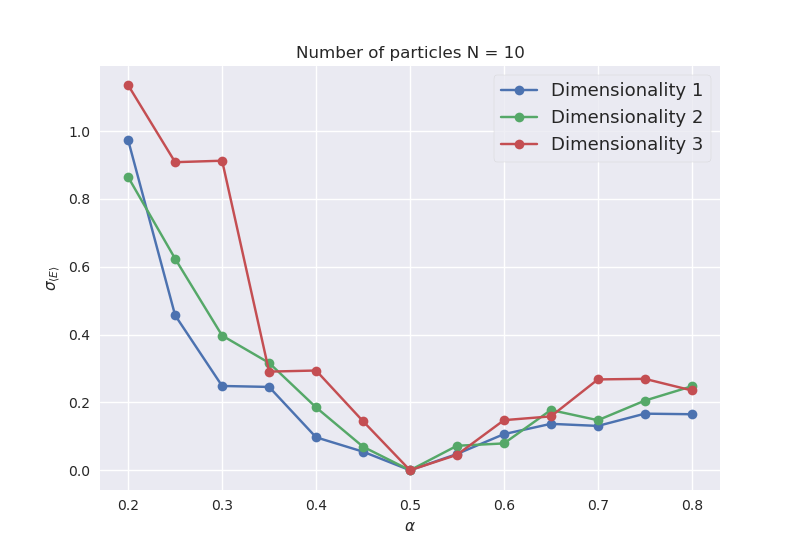
\includegraphics[scale=.5]{assets/plots/dim_and_n/std_10.0N.png}}\\
  \subfloat[]{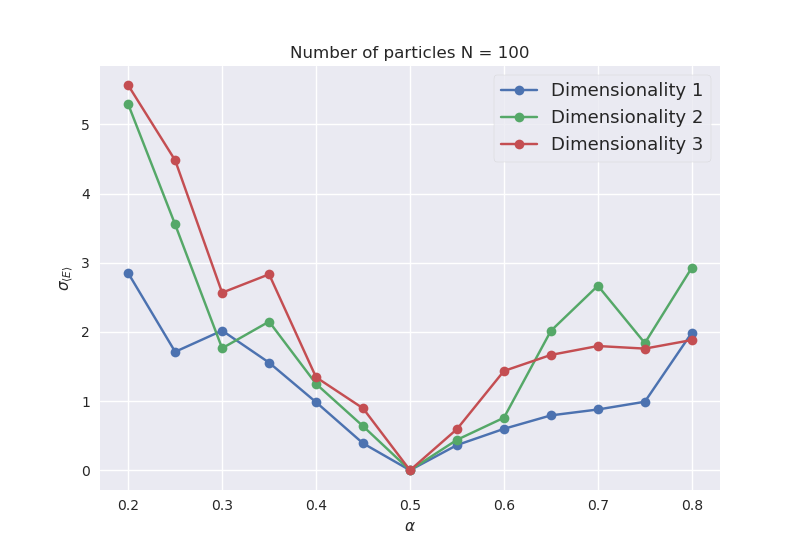
\includegraphics[scale=.5]{assets/plots/dim_and_n/std_100.0N.png}}
  \caption{Standard deviation over energy values generated on 8 cores simulatneously, for $N=1,10,100$ and $\dim=1,2,3$. The results show a staggeringly low standard deviation at the value of $\alpha = 0.5$. The system is non-interacting and the values are calculated with the brute force method.}
  \label{fig:optimal_alpha_std}
\end{figure}
\FloatBarrier

\hypertarget{steepest-gradient-descent-1}{%
\subsection{Steepest Gradient
Descent}\label{steepest-gradient-descent-1}}

Only the non-interacting case with 10 particles in 3 dimensions was
tested with 20 thousand Monte Carlo cycles. The first test was to see
what learning rate yielded sufficiently fast convergence to the correct
energy. The test was done with start \(alpha = 0.2\). The result can be
seen in figure \ref{fig:sgd-learning-rates} below.

\begin{figure}[ht]%
  \centerfloat
  \captionsetup[subfigure]{labelformat=empty}
  \subfloat[]{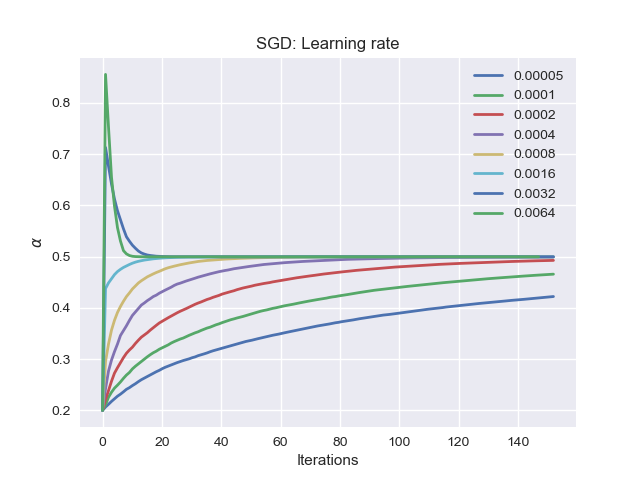
\includegraphics[scale=.5]{assets/plots/SGD_learning-rate.png}}
  \caption{Steepest gradient descent of start $\alpha = 0.2$ with different learning rates, $\eta$.}
  \label{fig:sgd-learning-rates}
\end{figure}
\FloatBarrier

This shows that a learning rate of \(0.0004\) is on the safe side of
stability, while still beeing fast enough. We then used this learning
rate for testing the convergence of our SGD to the correct \(\alpha\) by
starting at eight different alpha values:
\(\alpha = \{0.2, 0.3, 0.4, 0.5, 0.6, 0.7, 0.8, 0.9\}\). From figure
\ref{fig:sgd-alphas} below we see that the steepest gradient descent
method is executed beautifully as all starting values approaches the
correct \(\alpha\) value of \(0.5\).

\begin{figure}[ht]%
  \centerfloat
  \captionsetup[subfigure]{labelformat=empty}
  \subfloat[]{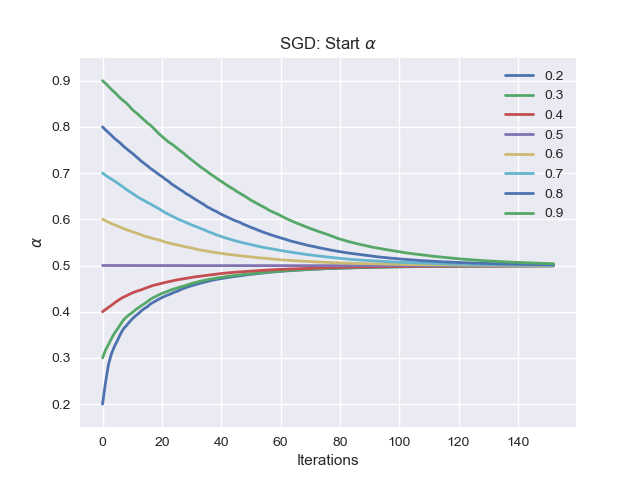
\includegraphics[scale=.5]{assets/plots/SGD_alphas.png}}
  \caption{Steepest gradient descent of different start $\alpha$.}
  \label{fig:sgd-alphas}
\end{figure}

\FloatBarrier

\hypertarget{an-interacting-system}{%
\subsection{An interacting system}\label{an-interacting-system}}

Following these tests for a non-interacting system, we put our solver to
the task of finding the energy of a system of \(10\) particles in an
elliptical harmonic potential (\(\beta = \gamma = 2.82843\)), at
different values of \(\alpha\) when the particles interact with
eachother. The results are shown in figure
\ref{fig:interacting-elliptical}.

\begin{figure}[htb]
  \centerfloat
  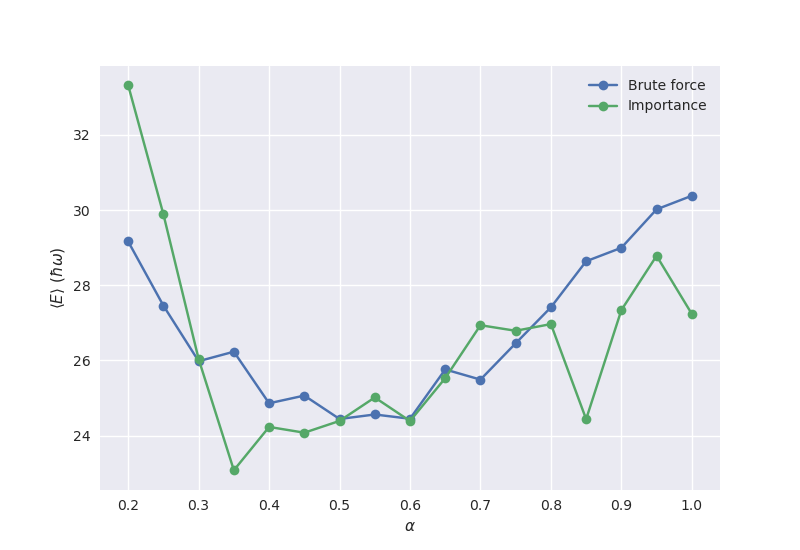
\includegraphics[scale=.5]{assets/plots/interacting_elliptical.png}
  \caption{The energy of a three-dimensional system of $10$ interacting particles, situated in an elliptical harmonic oscillator potential well. The energy is evaluated against different values of $\alpha$ and using the two Metropolis algorithms listed.}
  \label{fig:interacting-elliptical}
\end{figure}

They are quite ambigious, especially in the case of importance sampling.
After this, we ran our SGD solver with the same interacting system. This
yielded promising results under both Metropolis algorithms, both
converging on a value just below \(\alpha = 0.5\). However, as seen in
figure \ref{fig:sgd-interacting}, the brute force Metropolis algorithm
converges more quickly.

\begin{figure}[htb]
  \centerfloat
  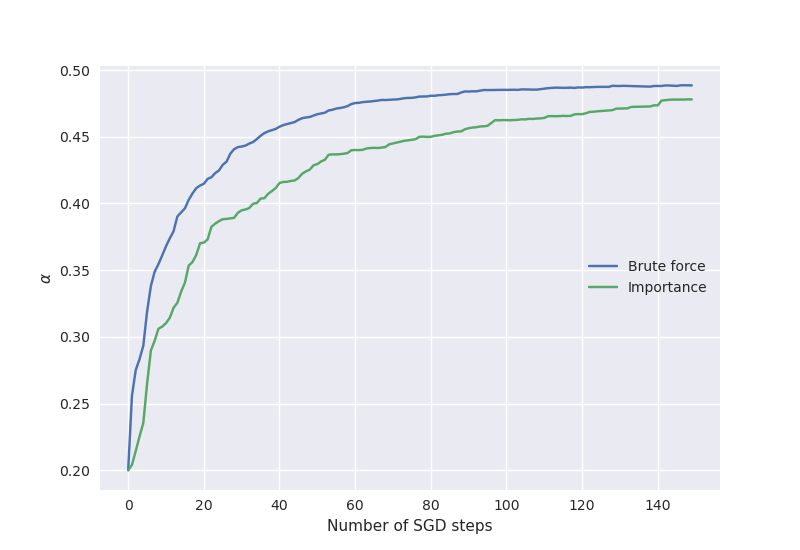
\includegraphics[scale=.5]{assets/plots/sgd_interacting.png}
  \caption{Convergence of $\alpha$ for the abovementioned system, solved using the two Metropolis algorithms listed. An acceptable convergence was aquired after $150$ steps, and so the SGD was stopped there for both algorithms.}
  \label{fig:sgd-interacting}
\end{figure}
\FloatBarrier

\hypertarget{discussion}{%
\section{Discussion}\label{discussion}}

\hypertarget{numerical-solver-compared-to-analytical-solutions}{%
\subsection*{Numerical solver compared to analytical
solutions}\label{numerical-solver-compared-to-analytical-solutions}}
\addcontentsline{toc}{subsection}{Numerical solver compared to
analytical solutions}

\hypertarget{local-energy}{%
\subsubsection*{Local energy}\label{local-energy}}
\addcontentsline{toc}{subsubsection}{Local energy}

The local energy for different alphas are shown in the figures
\ref{fig:BF_vs_IM_VS_analytical_1D}, \ref{fig:BF_vs_IM_VS_analytical_2D}
and \ref{fig:BF_vs_IM_VS_analytical_3D}. The plots originates from
caluclations utilizing the Brute Force Metropolis, Importance Sampling
and the analytical expression for the three dimensions and different
number of particles.

All the systems has one common point, namely \(\alpha = 0.5\). The two
numerical methods have, for most systems, an energy minima at this
point, which is expected.

Increasing the size of the sytem (higher number of dimensions and
particles) the energy approaches a more linear dependency of alpha. The
Importance Sampling method is aproaching linearity faster than the Brute
Force method. A possible explenation is decreasing accuracy for an
increasing size of the system, because the shape of the energy as a
function of alpha is expected to be a parabola. However, as can be seen,
the two numerical methods are also approaching the analytical values for
the energy for an increased size of the system.

Overall the analytical calulated energy is approximatly linear. However,
the expresson for the local energy (eq.
\eqref{eq:local-energy-gauss-scaled}) is proportional to \(\alpha^2\).
It is expected to be a parobola with an energy minima at
\(\alpha = 0.5\). Guessing there is something wrong with setup of the
particle positions.

\hypertarget{performance}{%
\subsubsection*{Performance}\label{performance}}
\addcontentsline{toc}{subsubsection}{Performance}

To measure the computational efficiency of the brute force Metropolis
and importance sampling algorithms, the elapsed time when calculating
energy for a specific \(\alpha\) (here \(\alpha = 0.5\)) was measured.
The times are listed in table \ref{tbl:BF_vs_IM_VS_analytical}. Its
worth noting that especially for the analytical calculations in lower
dimensions, writing to file and overhead from the Python runtime might
have affected the timing, as these calculations are very quick.

Looking at the greater picture, the computing time increased
proportionally with the number of dimensions and particles, as expected.
The brute force Metropolis method was faster than the importance
sampling method in all the measured computations. For the larger systems
of \(D = 2\) and \(3\), as well as \(N = 10\) to \(500\), the speedup is
approximately \(20- 25\%\) for the brute force Metropolis algorithm.

The results from the analytical measurement is another story. It is
orders of magnitude faster that the two numerical methods, as shown in
table \ref{tbl:BF_vs_IM_VS_analytical}. In the columns where the
computation time is \(0.0\) s, the computation was too fast to even get
a proper measurement. As the systems were calculated using different
setups/algorithms and because of a high inaccuracy in the measurment, no
further conclusions will be drawn from this result. However, it is
important to point out the fact that having an analytical expression for
the local energy will by it's nature give a significant calculation
speedup - seeing as we can simplify for whatever property we are looking
for. Having an analytical expression is an exception rather than a rule,
so for more complicated quantum mechanical systems, this would not be a
viable solution.

\hypertarget{brute-force-or-importance-sampling}{%
\subsection*{Brute force or importance
sampling}\label{brute-force-or-importance-sampling}}
\addcontentsline{toc}{subsection}{Brute force or importance sampling}

In our testing, the brute force Metropolis algorithm generally produced
better results, especially in terms of convergence, when employing
steepest gradient descent. This was surprising, and not in tune with our
expectations. The cause here is probably a poor implementation. We reach
the desired results by using importance sampling, but it's apparent that
we loose some accuracy throughout the algoritm. For further improving
this solver, this is the first issue that needs to be tackled, in order
to minimize the amount of Monte Carlo cycles needed to produce a
confident result.

\hypertarget{convergence-of-sgd}{%
\subsection*{Convergence of SGD}\label{convergence-of-sgd}}
\addcontentsline{toc}{subsection}{Convergence of SGD}

The convergence from different alphas to the correct one
(\(\alpha = 0.5\)) in figure \ref{fig:sgd-alphas} shows that the
convergence happens faster for \(\alpha\)-values below the correct one,
while higher \(\alpha\)-values converges slower. The reason for this is
that the derivative of the energy has a larger value when
\(\alpha < 0.5\), which by equation \eqref{eq:sgd} shows that the step
size is larger, in turn yielding faster convergence.

This being said, our SGD converged correctly and regardless of the
starting value of \(\alpha\), and thus works as expected.

\hypertarget{general-performance}{%
\subsection*{General performance}\label{general-performance}}
\addcontentsline{toc}{subsection}{General performance}

In general, the variational Monte Carlo solver yielded the desired
results confidently. By using Metropolis Monte Carlo integration
together with steepest gradient descent, we were able to produce the
correct optimal value of \(\alpha\) for both a non-interacting system
and an interacting one - with differing number of particles and
dimensionality.

\hypertarget{conclusion}{%
\section{Conclusion}\label{conclusion}}

Our variational Monte Carlo solver was successfully implemented and
finds the desired variational parameter \(\alpha\) per the specified
bosonic system, which is in accordance with the analytical solution.
Even though the solver provides correct results by utilizing importance
sampling in our Metropolis-Hastings algorithm, we experience
inconsistencies, slowdowns and errors with this method that were not
expected. This is emphasized as a topic of improvement for further
reports.

\clearpage
\appendix

\hypertarget{appendix}{%
\section{Appendix}\label{appendix}}

\hypertarget{source-code}{%
\subsection{Source code}\label{source-code}}

All source code for both the Rust VMC implementation and this document
is found in the following GitHub Repository

\url{https://github.com/kmaasrud/vmc-fys4411}

\hypertarget{notation-and-other-explanations}{%
\subsection{Notation and other
explanations}\label{notation-and-other-explanations}}

\hypertarget{index-notation-for-sums-and-products}{%
\subsubsection{Index notation for sums and
products}\label{index-notation-for-sums-and-products}}

For products and sums, the following convention is used:

\[\sum_{i <j}^N = \sum_{i=1}^N \sum_{j=i+1}^N,\quad \text{or}\quad \prod_{i <j}^N = \prod_{i=1}^N \prod_{j=i+1}^N\]

\hypertarget{calculations}{%
\subsection{Calculations}\label{calculations}}

\hypertarget{second-derivative-of-trial-wave-function}{%
\subsubsection{Second derivative of trial wave
function}\label{second-derivative-of-trial-wave-function}}

\[
\begin{aligned}
\nabla_{i}^2 \Psi_{T}(\mathbf{r})
&= \nabla_{i} \cdot\left[\frac{\partial}{\partial x_{i}}, \frac{\partial}{\partial y_{i}},   
   \frac{\partial}{\partial z_{i}}\right] \Psi_{T}(\mathbf{r}) \\
&= \nabla_i \cdot \left[\frac{\partial}{\partial x_i} \exp{(-\alpha
   \mathbf{r}_i^2}),\frac{\partial}{\partial y_i} \exp{(-\alpha \mathbf{r}_i^2}), \frac{\partial}{\partial z_i} \exp{(-\alpha \mathbf{r}_i^2})\right] \\
&= \nabla_{i} \cdot \left[-2 \alpha x_{i} \exp{(-\alpha \mathbf{r}_{i}^{2}}), -2 \alpha
   y_{i}  
   \exp{(-\alpha \mathbf{r}^2_{i}}), -2 \alpha z_{i} \exp{(-\alpha \mathbf{r}_{i}^2})
   \right] \\
&= -2 \alpha \left[  \exp{(-\alpha \mathbf{r}^2_{i}})(1 - 2 \alpha x^2_{i}), \exp{(-\alpha
   \mathbf{r}^2_{i}})(1 - 2 \alpha y^2_{i}), \exp{(-\alpha \mathbf{r}^2_{i}})
   (1 - 2 \alpha z^2_{i}) \right] \\
&= -2\alpha \Psi_{T} \left[(1 - 2 \alpha x^2_{i}), (1 - 2 \alpha y^2_{i}),
   (1 - 2 \alpha  z^2_{i}) \right]\\
&= -2\alpha \Psi_{T}\sum_{d = x,y,z}1 -2\alpha d_{i}^2 \\
&= -2\alpha \Psi_{T}(\dim - 2 \alpha  \mathbf{r}^2_{i})
\end{aligned}
\]

\hypertarget{local-energy-for-gaussian-wave-function}{%
\subsubsection{Local energy for Gaussian wave
function}\label{local-energy-for-gaussian-wave-function}}

Starting with

\[
E_L(\mathbf{r}) =
    \frac{1}{\Psi_T(\mathbf{r})} \left[ \sum_i^N \left (\frac{-\hbar^2}{2m}
    \nabla_{i}^2 \Psi_T (\mathbf{r}) + V_\text{ext} ({\mathbf{r}}_i) \Psi_T(\mathbf{r}) \right)  
    \right],
\]

and using the result from
\ref{second-derivative-of-trial-wave-function}, this results in:

\[
\begin{aligned} E_L (\mathbf r) &=  \frac{1}{\Psi_T(\mathbf{r})}  \left[ \sum_i^N \left(  \frac{\hbar^2 \alpha}{m}  (\dim - 2
    \alpha  \mathbf{r}^2_{i} ) + \frac{1}{2} m \omega^2_\text{ho} \mathbf{r}^2_{i} \right) \Psi_T(\mathbf{r}) \right ]\\
&= \frac{\hbar^2 }{m} \alpha N \dim +  \left( \frac{1}{2} m \omega^2_\text{ho} - 2 \alpha^2\right)  \sum_i^N \mathbf{r}^2_{i}
\end{aligned}
\]

\hypertarget{sec:trial_wf_gradient}{%
\subsubsection{Gradient of interacting trial wave
function}\label{sec:trial_wf_gradient}}

Rewriting the wave function to

\[
\Psi_T(\mathbf{r})=\left[
    \prod_i^N \phi(\mathbf{r}_i)
\right]
\exp{\left(\sum_{i<j}u(r_{ij})\right)}
\]

where \(r_{ij} = |r_i - r_j|\) and we set \(u(r_{ij}) = \ln f(r_{ij})\).
Lastly \(g(\alpha, \beta,\mathbf{r}_i)\) is redefined to the following
function

\[
\phi(\mathbf{r}_i) = \exp [-\alpha(x_i^2 + y_i^2 + \beta z_i^2)] = g(\alpha, \beta,\mathbf{r}_i).
\]

For convenience

\[ \Psi_1 (\mathbf{r}_{i})= \prod_i^N \phi(\mathbf{r}_i)\]

and

\[\Psi_2 (\mathbf{r}_ {ij}) = \exp{\left(\sum_{i<j}u(r_{ij})\right)}\]

where \(\Psi_1\) and \(\Psi_2\) is the one-body and correlated part of
the wave function, respectively. Both parts have simple dependency of
the k'th particle. \(\Psi_1\) is a product of one-body wave functions
with only one factor dependent of \(\mathbf{r}_k\) and \(\Psi_2\) is
\(\mathbf{r}_k\) - dependent for the pairs
\(\sum _{i\ne k} u(\mathbf{r} _{ik})\). Hence the first derivatives
becomes

\[
\nabla_k \Psi_1(\mathbf{r}) = \left[\prod_ {i\ne k}^N \phi(\mathbf{r}_i) \right] \nabla_k \phi(\mathbf{r}_k)
\]

\[
\nabla_k \Psi_2(\mathbf{r}_ {ij}) = \exp {\left (\sum_ {i<j}u(r_{ij})\right)}  \sum_ {i \ne k} \nabla_k  u(\mathbf{r}_{ik})
\]

Giving the first derivate of the trail wave function

\[
\nabla_k \Psi_T(\mathbf{r}) = \nabla_k \phi(\mathbf{r}_ k) \left [\prod_ {i\ne k}^N \phi(\mathbf{r}_ i) \right] \exp {\left (\sum_ {i<j}u(r_{ij})\right)} \\ +
 \prod_i^N \phi (\mathbf{r}_ i) \exp{ \left( \sum_{i<j} u(r_{ij}) \right)}  \sum_ {i \ne k} \nabla_k  u(\mathbf{r}_{ik})
\]

\hypertarget{sec:trial_wf_laplacian}{%
\subsubsection{Laplacian of interacting trial wave
function}\label{sec:trial_wf_laplacian}}

The Laplacian of the wacefunction needs to be evaluated in order to
calculate

\[
\frac{1}{\Psi_T(\mathbf {r})} \nabla_k \nabla_k \Psi_T(\mathbf{r})
\]

The last part, \(\nabla_k \Psi_T(\mathbf{r})\) is calculated in the
section above / equation (\textbf{Reference here}). Next step is then to
calculate

\begin{align*}
\nabla_k \nabla_k \Psi_T(\mathbf{r}) = &\nabla_k \bigg( \nabla_k \phi(\mathbf r_k) \left [\prod_{i\ne k} \phi(\mathbf r_i) \right] \exp{\left (\sum_{j<m}u(r_{jm})\right)} \\
 &+ \prod_i \phi (\mathbf r_i) \exp{\left(\sum_{j<m} u(r_{jm}) \right)}  \sum_{l \ne k} \nabla_k  u(\mathbf r_{kl}) \bigg) \\
\nabla_k \nabla_k \Psi_T(\mathbf r) = &\prod_{i\ne k} \left[ \nabla_k^2 \phi(\mathbf r_k) \exp{\left(\sum_{j<m} u(r_{jm})\right)} + \nabla_k \phi(\mathbf r_k) \cdot  \nabla_k \exp{\left( \sum_{j < m} u(r_{jm})\right)} \right] \\ &+ \nabla_k \prod_i \phi (\mathbf r_i) \exp{\left (\sum _{j<m} u(r_{jm})\right)}\sum_{l \ne k} \nabla_k u(r_{kl}) \\ &+
\nabla_k \exp{\left(\sum_{j < m} u(r_{jm})\right)}\prod_i \phi(\mathbf{r}_i) \sum_{l \ne k} \nabla_k u(r_{kl}) \\ &+ \nabla_k \sum_{l \ne k} \nabla_k u (r_{kl}) \prod_i \phi (\mathbf{r}_i) \exp{\sum_{j < m} u (r_{jm})}
\end{align*}

In order to avoid writing long calculations, the three main gradients
are calculated below. The last of the three following
expressions/equations is a bit more of a hazard to calculate. First the
product rule is used. Then a rule for the gradient is applied where the
gradient of a unit vector is 2 divided by its magnitude. \(u'\) is
parallel to the unit vector, hence their product becomes a scalar, the
second derivate of \(u\).

\[
\nabla_k
\exp{\left(\sum_{j <m}{u(r_{jm}}\right)} = \exp{\left(\sum_{j <m}{u(r_{jm}}\right)} \sum_{l \ne k}{\nabla_k u(r_{kl})}
\]

\[
\nabla_k \prod_i \phi(\mathbf{r}_i) = \prod _{i \ne k} \phi(\mathbf{r}_i) \nabla_k \phi(\mathbf {r}_k)
\]

\begin{align*}
\nabla_k \sum_{l \ne k}{\nabla_k u(r_{kl})} &= \sum_{l \ne k}{\nabla_k \left(\frac{\mathbf{r}_l - \mathbf {r}_k}{\mathbf{r} _{lk}} u'(r _{lk})\right)} \\ &= \sum _{l\ne k}\left(\nabla_k \frac{\mathbf{r}_l - \mathbf {r}_k}{\mathbf{r} _{lk}} u'(r _{lk}) + \frac{\mathbf{r}_l - \mathbf {r}_k}{\mathbf{r} _{lk}} \nabla_k u'(r _{lk}) \right) \\ &= \sum _{l\ne k} \frac{2}{r _{lk}} + u''(r _{lk})
\end{align*}

Finally the Laplacian can be calculated, by reintroducing the fraction
\(\frac{1}{\Psi_T(\mathbf{r})}\)

\begin{align*}
\frac{1}{\Psi_T(\mathbf{r})} \nabla_k^2 \Psi_T(\mathbf{r}) = &\frac{\prod_{i \ne k} \phi(\mathbf{r}_i)}{\prod _{i} \phi(\mathbf{r}_i)} \left(\nabla^2_k \phi(\mathbf{r}_k) + \nabla_k \phi(\mathbf{r}_k \sum _{l\ne k}\nabla_k u(r _{kl})\right)  + \left( \frac{\nabla_k \phi(\mathbf{r}_i)}{\phi(\mathbf{r}_i)} \sum _{l \ne k} \nabla_k u(r _{kl})\right) \\ &+ \sum _{l \ne k} \nabla_k u(r _{kl})  + \sum _{j \ne k} \nabla_k u(r _{kj}) + \nabla_k  \sum _{l \ne k} \nabla_k u(r _{kl})
\end{align*}

The second and third terms are the same. Two of the terms are shown in
the calculations above and \(\nabla_k u(r_{kl})\) is the unit vector
multiplied with the derivate of a scalar. Then we have the final
expression

\begin{align*}
\frac{1}{\Psi_T(\mathbf{r})} \nabla_k^2 \Psi_T(\mathbf{r}) = &\frac{\nabla_k \phi(\mathbf{r}_k)}{\phi(\mathbf{r}_k)} + 2 \frac{\nabla_k \phi(\mathbf{r}_k)}{\phi(\mathbf{r}_k)}\sum _{j\ne k}
\frac{\mathbf{r}_j - \mathbf {r}_k}{\mathbf{r} _{jk}}u'(r _{lk}) \\ &+ \sum _{j\ne k}\sum _{l\ne k}
\frac{\mathbf{r}_j - \mathbf {r}_k}{\mathbf{r} _{jk}} u'(r _{lk}) + \sum _{j\ne k}\sum _{l\ne k}
\frac{\mathbf{r}_j - \mathbf {r}_k}{\mathbf{r} _{jk}} \frac{\mathbf{r}_l - \mathbf {r}_k}{\mathbf{r} _{lk}}  u'(r _{jk})  u'(r _{lk}) \\ &+ \sum _{l\ne k} \frac{2}{r _{lk}} u'(r _{lk}) +  u''(r _{lk})
\end{align*}

\hypertarget{sec:scaled_ham}{%
\subsubsection{Scaling of repulsion Hamiltonian}\label{sec:scaled_ham}}

We have the initial expression for the Hamiltonian,
\eqref{eq:hamiltonian}. Inserting \eqref{eq:external-potential}, we get:

\[ H = \frac{1}{2}\sum_i^N \left(-\frac{\hbar^2}{m}\nabla^2_i + m\left(\omega_\text{ho}^2 (r_{x, i}^2 + r_{y, i}^2) + \omega_z^2 r_{z, i}^2\right)\right) + \sum_{i<j}^N V_\text{int}(|\mathbf r_i - \mathbf r_j|) .\]

We now introduce the scaled length unit \(r' = \frac{r}{a_\text{ho}}\)
which in turn leads to
\(\nabla^{\prime 2}_i = a_\text{ho}^2\nabla_i^2\).

\[ H = \frac{1}{2}\sum_i^N \left(-\frac{\hbar^2}{ma_\text{ho}^2}\nabla^{\prime 2}_i  + ma_\text{ho}^2\left(\omega_\text{ho}^2(r_{x, i}^{\prime 2} + r_{y, i}^{\prime 2}) + \omega_z^2 r_{z, i}^{\prime 2}\right)\right) + \sum_{i<j}^N V_\text{int}(|\mathbf r_i - \mathbf r_j|)\]

Inserting the definition of
\(a_\text{ho} = \frac{\hbar}{m\omega_\text{ho}}\), we get

\[ H = \frac{1}{2}\sum_i^N \left(-\hbar\omega_\text{ho}\nabla^{\prime 2}_i  + \hbar\omega_\text{ho}\left((r_{x, i}^{\prime 2} + r_{y, i}^{\prime 2}) + \frac{\omega_z^2}{\omega_\text{ho}^2} r_{z, i}^{\prime 2}\right)\right) + \sum_{i<j}^N V_\text{int}(|\mathbf r_i - \mathbf r_j|), \]

\[ H = \frac{\hbar\omega_\text{ho}}{2}\sum_i^N \left(-\nabla^{\prime 2}_i  + (r_{x, i}^{\prime 2} + r_{y, i}^{\prime 2}) + \gamma^2 r_{z, i}^{\prime 2})\right) + \sum_{i<j}^N V_\text{int}(|\mathbf r_i - \mathbf r_j|), \]

where \(\gamma = \frac{\omega_z}{\omega_\text{ho}}\). We lastly
reorganize the above to obtain a scaled Hamiltonian
\(H' = \frac{H}{\hbar\omega_\text{ho}}\) and also make sure to scale the
function \(V_\text{int}\rightarrow V'_\text{int}\) by transitioning from
\(a\rightarrow a' = \frac{a}{a_\text{ho}}\).

\begin{equation} H' = \frac{1}{2}\sum_i^N \left(-\nabla_i^{\prime 2} + r_{x, i}^{\prime 2} + r_{y, i}^{\prime 2} + \gamma^2 r_{z, i}^{\prime 2}\right) + \sum_{i<j}^N V'_\text{int}(|\mathbf r'_i - \mathbf r'_j|) .\label{eq:scaled_ham_appendix}\end{equation}

By ensuring that we used scaled length units of
\(r' = \frac{r}{a_\text{ho}}\) and scaled energy units of
\(E' = \frac{E}{\hbar\omega_\text{ho}}\), equation
\eqref{eq:scaled_ham_appendix} holds. For simplification, we will not
use the primed notation outside this derivation.

\hypertarget{bibliography}{%
\section*{References}\label{bibliography}}
\addcontentsline{toc}{section}{References}

\hypertarget{refs}{}
\begin{CSLReferences}{0}{0}
\leavevmode\vadjust pre{\hypertarget{ref-DuBoisGlyde2001}{}}%
\CSLLeftMargin{{[}1{]} }
\CSLRightInline{J. L. DuBois and H. R. Glyde, {``Bose-einstein
condensation in trapped bosons: A variational monte carlo analysis,''}
\emph{Phys. Rev. A}, vol. 63, p. 023602, Jan. 2001, doi:
\href{https://doi.org/10.1103/PhysRevA.63.023602}{10.1103/PhysRevA.63.023602}.}

\leavevmode\vadjust pre{\hypertarget{ref-Griffiths}{}}%
\CSLLeftMargin{{[}2{]} }
\CSLRightInline{David. J. Griffiths, \emph{Introduction to Quantum
Mechanics}. 2005.}

\leavevmode\vadjust pre{\hypertarget{ref-Project1}{}}%
\CSLLeftMargin{{[}3{]} }
\CSLRightInline{M. Hjorth-Jensen, {``Project 1.''} Jan. 2021.}

\leavevmode\vadjust pre{\hypertarget{ref-CompQuantum2020}{}}%
\CSLLeftMargin{{[}4{]} }
\CSLRightInline{M. Hjorth-Jensen, \emph{{Advanced Topics in
Computational Physics: Computational Quantum Mechanics}}. 2020.}

\leavevmode\vadjust pre{\hypertarget{ref-AasrudRongveRaniseth2019}{}}%
\CSLLeftMargin{{[}5{]} }
\CSLRightInline{K. M. Aasrud, A. S. Rongve, and A. M. Raniseth,
{``Project 3.''} Oct. 2019, {[}Online{]}. Available:
\url{https://github.com/kmaasrud/gq-mcm-fys3150/blob/master/doc/Project-3_Aasrud-Raniseth-Rongve.pdf}.}

\leavevmode\vadjust pre{\hypertarget{ref-Nilsen2008}{}}%
\CSLLeftMargin{{[}6{]} }
\CSLRightInline{J. K. Nilsen, {``Data blocking - FYS4410 lecture.''}
2008, {[}Online{]}. Available:
\url{https://www.uio.no/studier/emner/matnat/fys/nedlagte-emner/FYS4410/v08/undervisningsmateriale/Material\%20for\%20Part\%20I\%20by\%20Morten\%20HJ/Slides\%20from\%20Lectures/blocking.pdf}.}

\leavevmode\vadjust pre{\hypertarget{ref-rustc_book}{}}%
\CSLLeftMargin{{[}7{]} }
\CSLRightInline{Rust Community, {``The rustc book.''} {[}Online{]}.
Available: \url{https://doc.rust-lang.org/rustc/}.}

\end{CSLReferences}

\end{document}
